\documentclass[compress]{beamer}
\usepackage{ifthen,verbatim}

\newcommand{\isnote}{}
\xdefinecolor{lightyellow}{rgb}{1.,1.,0.25}
\xdefinecolor{darkblue}{rgb}{0.1,0.1,0.7}

%% Uncomment this to get annotations
%% \def\notes{\addtocounter{page}{-1}
%%            \renewcommand{\isnote}{*}
%% 	   \beamertemplateshadingbackground{lightyellow}{white}
%%            \begin{frame}
%%            \frametitle{Notes for the previous page (page \insertpagenumber)}
%%            \itemize}
%% \def\endnotes{\enditemize
%% 	      \end{frame}
%%               \beamertemplateshadingbackground{white}{white}
%%               \renewcommand{\isnote}{}}

%% Uncomment this to not get annotations
\def\notes{\comment}
\def\endnotes{\endcomment}

\setbeamertemplate{navigation symbols}{}
\setbeamertemplate{headline}{\mbox{ } \hfill
\begin{minipage}{5.5 cm}
\vspace{-0.75 cm} \small
\end{minipage} \hfill
\begin{minipage}{4.5 cm}
\vspace{-0.75 cm} \small
\begin{flushright}
\ifthenelse{\equal{\insertpagenumber}{1}}{}{Jim Pivarski \hspace{0.2 cm} \insertpagenumber\isnote/\pageref{numpages}}
\end{flushright}
\end{minipage}\mbox{\hspace{0.2 cm}} \hspace{0.01 cm} \vspace{-1.05 cm}}

\newcommand{\s}[1]{{\mbox{\scriptsize #1}}}

\begin{document}
\begin{frame}
\vfill
\begin{center}
\textcolor{darkblue}{\Large Dark Matter and Dark Energy}

\vfill
\begin{columns}
\column{0.3\linewidth}
\begin{center}
\large
Jim Pivarski
\end{center}
\end{columns}

%% \begin{columns}
%% \column{0.3\linewidth}
%% \begin{center}
%% \scriptsize
%% {\it Fermilab}
%% \end{center}
%% \end{columns}

\vfill
March 4, 2012

\end{center}
\end{frame}

%% \begin{notes}
%% \item This is the annotated version of my talk.
%% \item If you want the version that I am presenting, download the one
%% labeled ``slides'' on Indico (or just ignore these yellow pages).
%% \item The annotated version is provided for extra detail and a written
%% record of comments that I intend to make orally.
%% \item Yellow notes refer to the content on the {\it previous} page.
%% \item All other slides are identical for the two versions.
%% \end{notes}

\small

%% \begin{frame}
%% \frametitle{Outline}

%% %% \begin{itemize}\setlength{\itemsep}{0.75 cm}
%% %% \item 
%% %% \end{itemize}
%% %% \hspace{-0.83 cm} \textcolor{darkblue}{\Large Outline2}
%% \end{frame}

%% \section*{First section}
%% \begin{frame}
%% \begin{center}
%% \Huge \textcolor{blue}{First section}
%% \end{center}
%% \end{frame}

\section*{Introduction}

\begin{frame}
\vspace{-2.3 cm}
\mbox{\hspace{-7 cm} 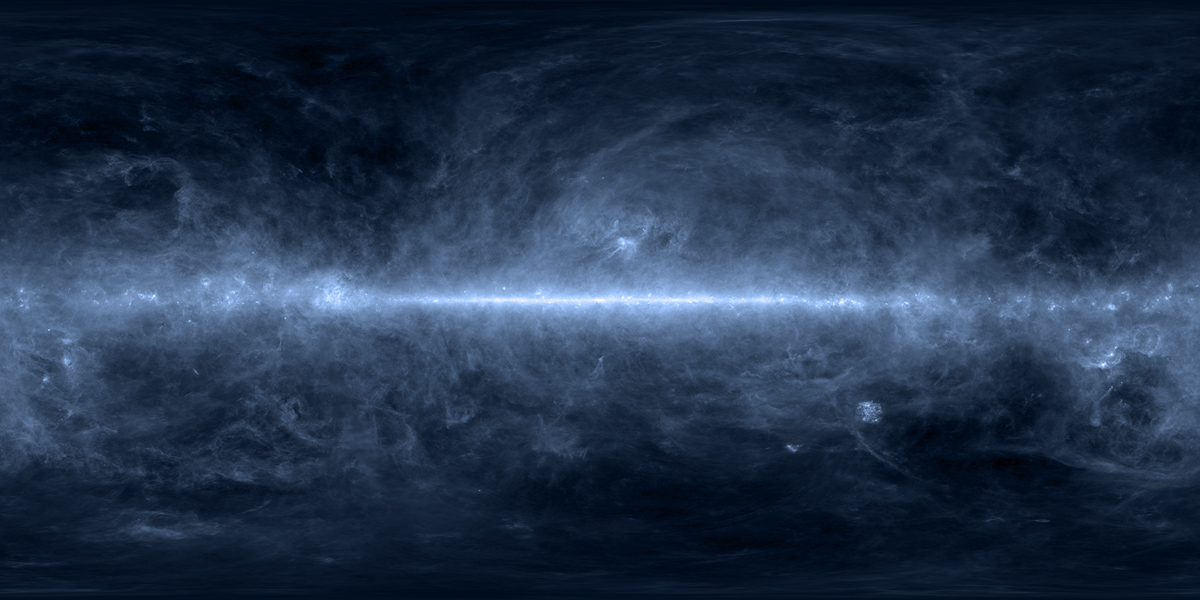
\includegraphics[width=1.85\linewidth]{pictures/spacedust.jpg}}
% http://www.cosmotography.com/images/galactic_cirrus.html

\vspace{-6.3 cm}
\begin{center}
\begin{minipage}{0.8\linewidth}
\textcolor{white}{\Huge Matter as we know it is}

\vspace{0.4 cm}
\textcolor{white}{\Huge a minority of the universe.}
\end{minipage}
\end{center}
\end{frame}

\begin{frame}
\begin{center}
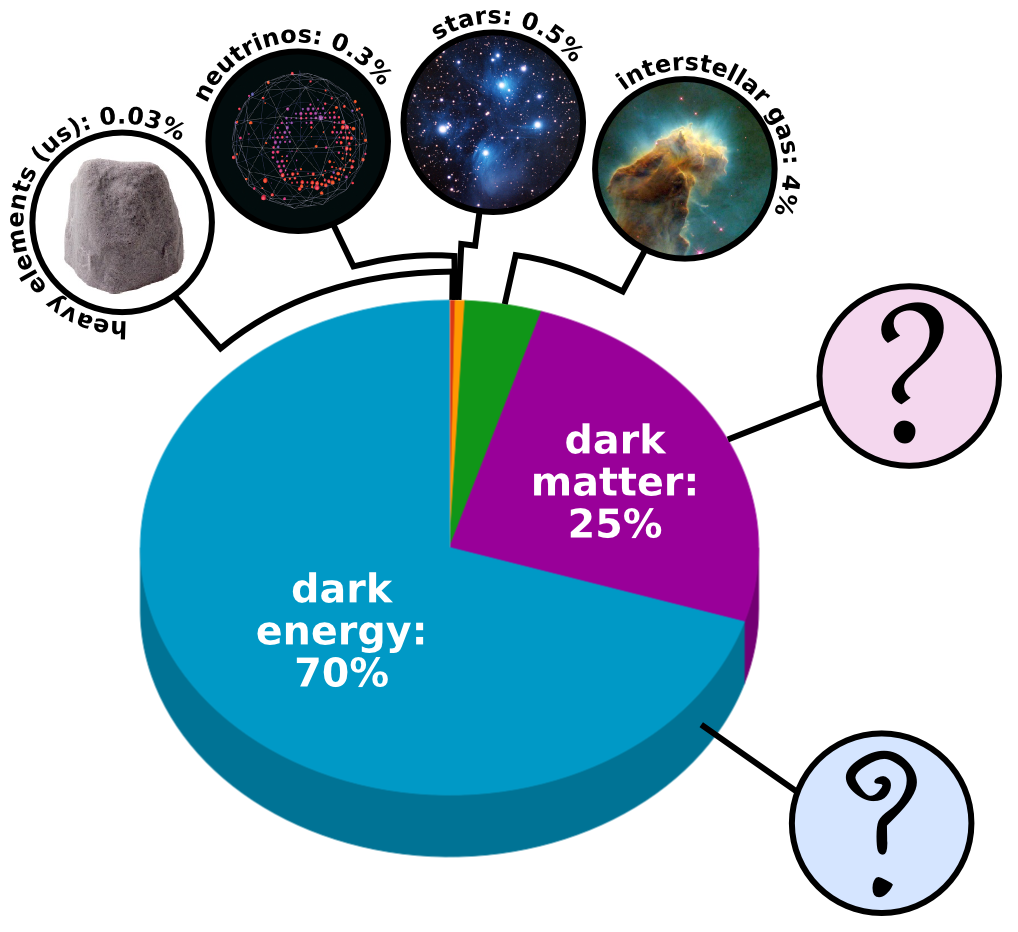
\includegraphics[width=0.95\linewidth]{pictures/piechart.png}
\end{center}
\end{frame}

\begin{frame}
\begin{center}
\begin{minipage}{0.9\linewidth}
\vspace{0.5 cm}
\textcolor{darkblue}{\huge This talk:}

\Large
\vspace{0.5 cm}
\begin{itemize}\setlength{\itemsep}{0.5 cm}
\item What is dark matter?
\begin{itemize}
\item The astronomer's toolbox: how we measure the sky
\item More mass than expected
\item What is it? (narrowing the options)
\end{itemize}

\item What is dark energy?
\begin{itemize}
\item How space-time curves
\item Expansion of the universe
\item Accelerating expansion: what is it???
\end{itemize}
\end{itemize}

\end{minipage}
\end{center}
\end{frame}

\section*{The Astronomer's Toolbox}

\begin{frame}
\frametitle{The astronomer's toolbox}

\mbox{\hspace{-0.75 cm} 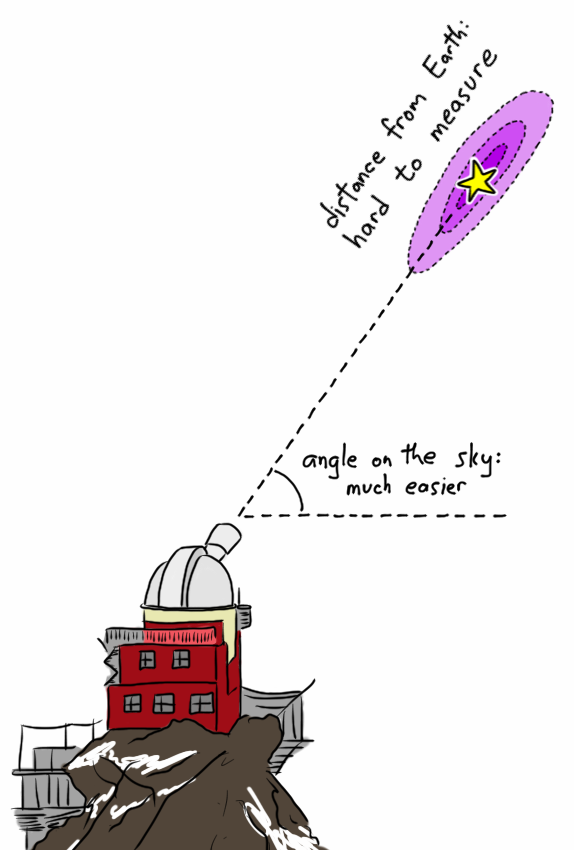
\includegraphics[height=8 cm]{pictures/measure_position.png}
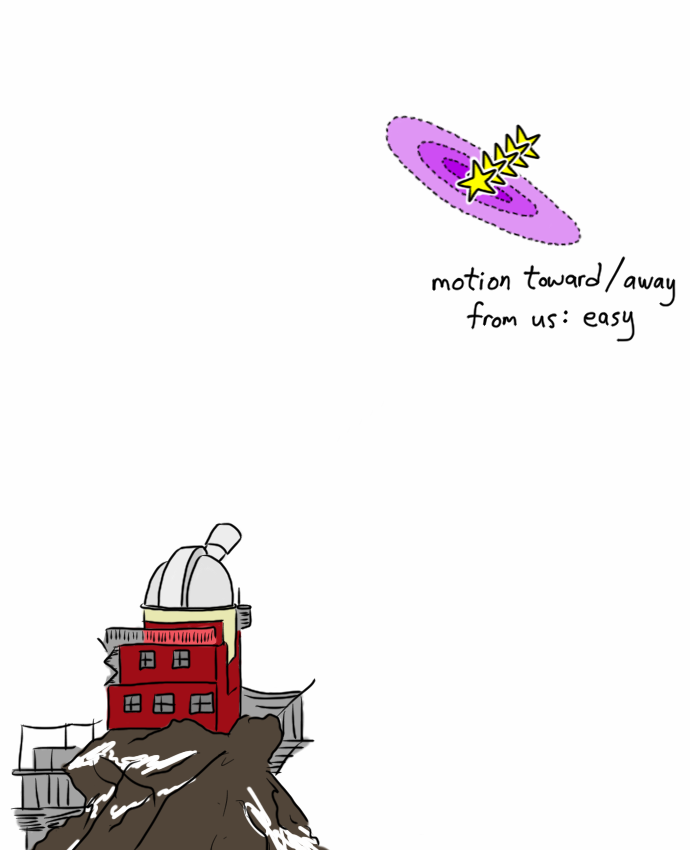
\includegraphics[height=8 cm]{pictures/measure_velocity.png}}
\end{frame}

\begin{frame}
\frametitle{The astronomer's toolbox}
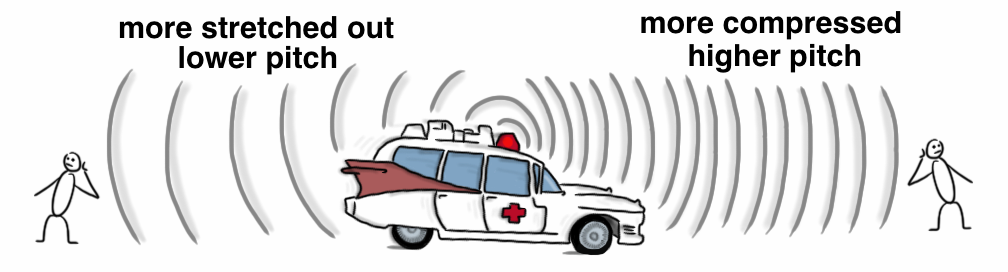
\includegraphics[width=\linewidth]{pictures/ambulance.png}

\vfill
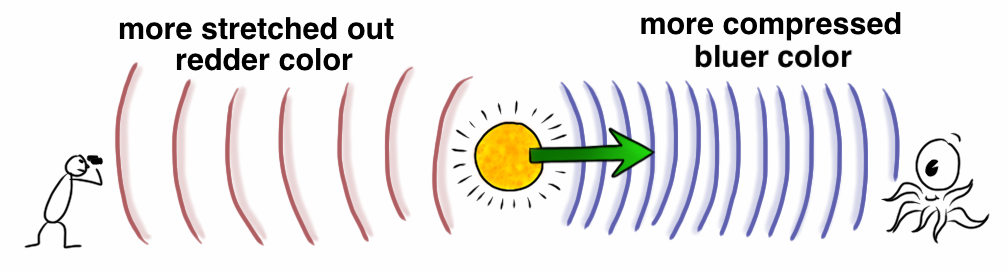
\includegraphics[width=\linewidth]{pictures/redshift_blueshift.png}

By comparing the observed color of the star with its actual color, we
can determine how fast it's moving.

\uncover<2>{\textcolor{darkblue}{But how do we know the actual color of the star?}}
\end{frame}

\begingroup
\setbeamercolor{background canvas}{bg=black}
\begin{frame}
\frametitle{\textcolor{white}{Chemical fingerprints}}
\begin{center}
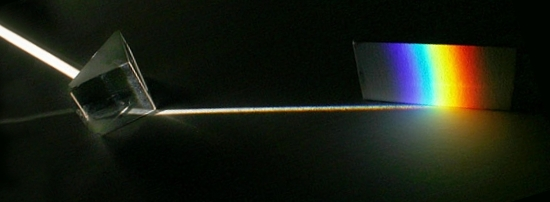
\includegraphics[width=0.5\linewidth]{pictures/prism.jpg}

\textcolor{white}{Every element has a unique set of spectral lines.}

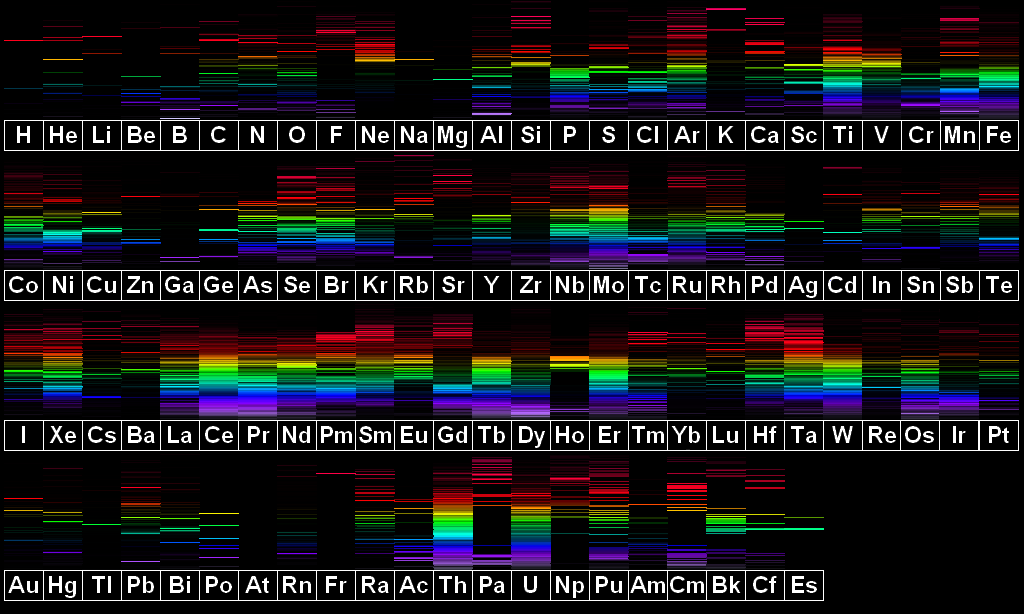
\includegraphics[width=0.9\linewidth]{pictures/spectral_tableofelements.png}
\end{center}
\end{frame}

\begin{frame}
\frametitle{\textcolor{white}{Chemical fingerprints}}
\begin{columns}
\column{0.55\linewidth}

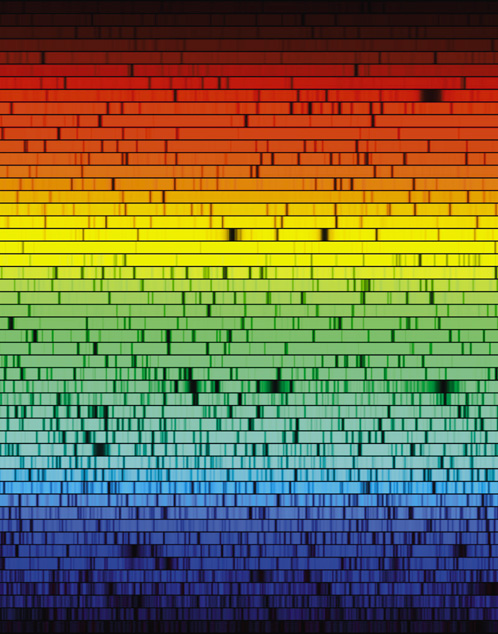
\includegraphics[width=\linewidth]{pictures/solarspectrum.jpg}

\centering \Large \textcolor{white}{The Sun}

\column{0.45\linewidth}
\textcolor{white}{The spectrum of each star is a combination of these lines, in proportion to the abundance of the elements in the star.}

\vspace{0.25 cm}
\textcolor{white}{If the star is moving toward or away from us, the whole spectrum is merely shifted to the right (bluer) or the left (redder).}

\vspace{0.25 cm}
\textcolor{white}{The combinations of lines are distinct enough to be recognized in spite of the shift.}

\end{columns}
\end{frame}
\endgroup

\begin{frame}
\frametitle{Another tool: measuring mass}
\begin{columns}
\column{0.4\linewidth}
\begin{minipage}{6.5 cm}
Astronomers can measure the mass of celestial objects whether they are
visible or not.
\end{minipage}

\vspace{0.25 cm}
\begin{minipage}{5.5 cm}
Mass bends space-time, distorting the paths of
light rays from background stars and galaxies.
\end{minipage}

\vspace{0.25 cm}
\begin{minipage}{5 cm}
On earth, we see multiple images or even connected rings of the
background galaxies.
\end{minipage}

\vspace{0.25 cm}
\only<1>{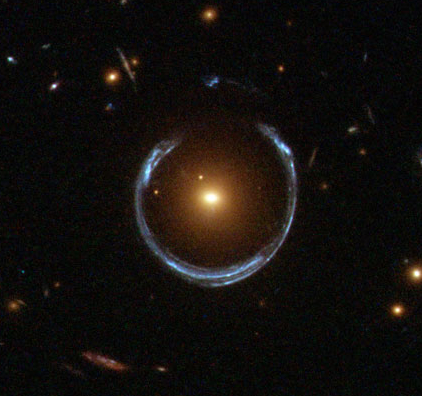
\includegraphics[width=\linewidth]{pictures/einstein_ring_real.jpg}}
\only<2>{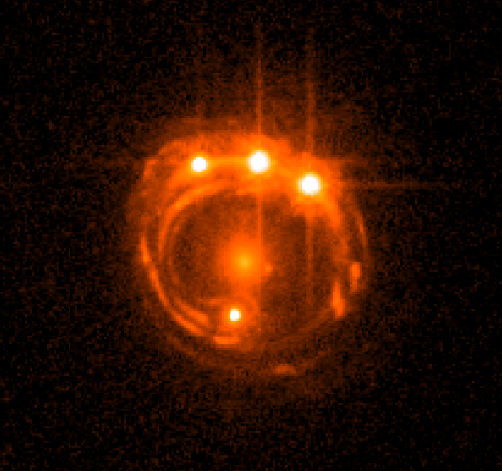
\includegraphics[width=\linewidth]{pictures/einstein_ring_real2.png}}

\column{0.6\linewidth}
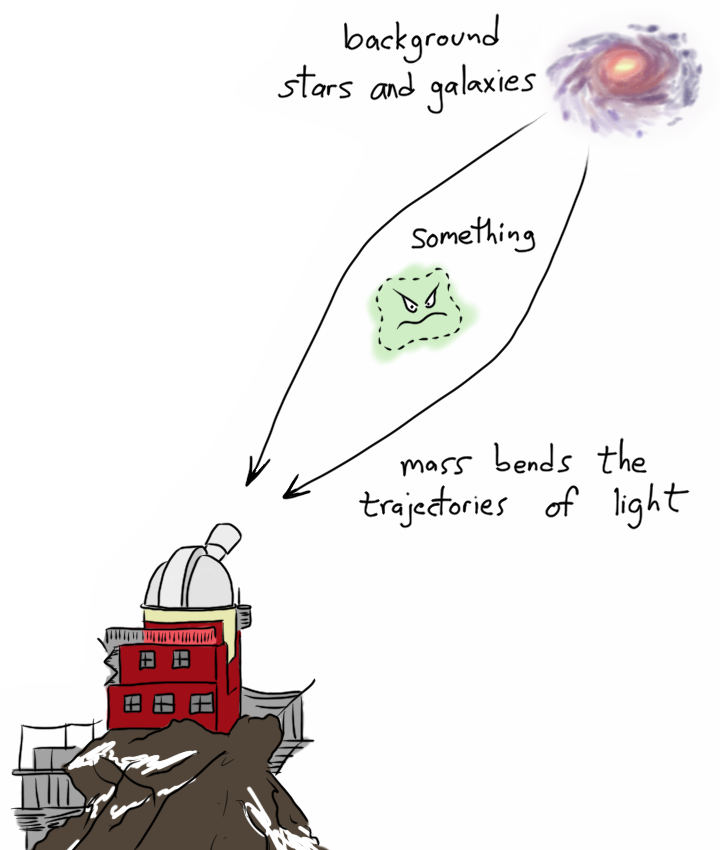
\includegraphics[height=8 cm]{pictures/lensing.png}
\end{columns}
\end{frame}

\begin{frame}
\frametitle{Simulated lensing of a black hole}

\begin{tabular}{p{0.3\linewidth} p{0.3\linewidth} p{0.3\linewidth}}
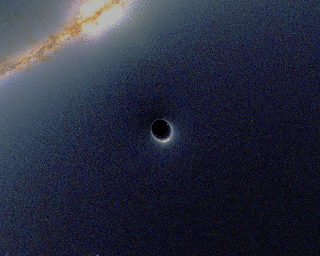
\includegraphics[width=\linewidth]{pictures/black_hole_lensing1.png} &
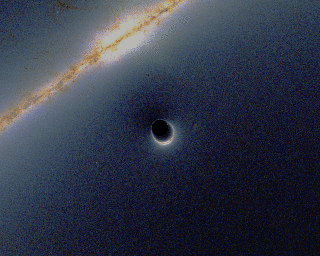
\includegraphics[width=\linewidth]{pictures/black_hole_lensing2.png} &
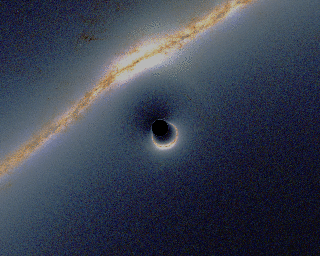
\includegraphics[width=\linewidth]{pictures/black_hole_lensing3.png} \\
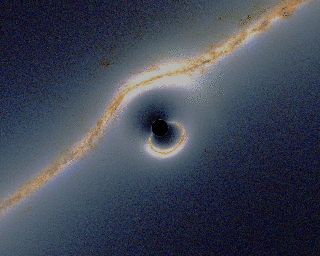
\includegraphics[width=\linewidth]{pictures/black_hole_lensing4.png} &
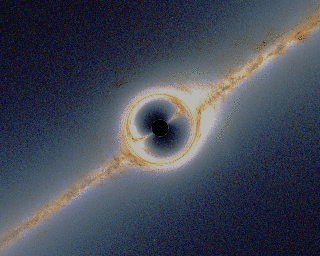
\includegraphics[width=\linewidth]{pictures/black_hole_lensing5.png} &
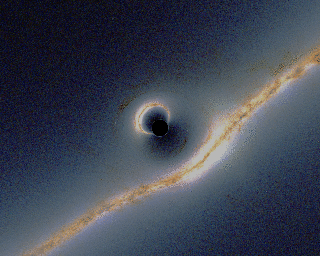
\includegraphics[width=\linewidth]{pictures/black_hole_lensing6.png} \\
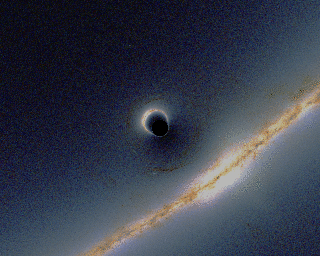
\includegraphics[width=\linewidth]{pictures/black_hole_lensing7.png} &
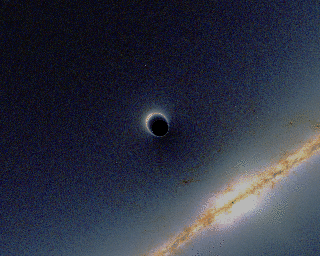
\includegraphics[width=\linewidth]{pictures/black_hole_lensing8.png} &
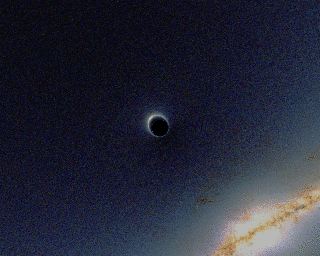
\includegraphics[width=\linewidth]{pictures/black_hole_lensing9.png}
\end{tabular}
\end{frame}

\section*{Dark Matter}
\begin{frame}
\begin{center}
\Huge \textcolor{blue}{Dark Matter}
\end{center}
\end{frame}

\begin{frame}
\frametitle{Testing gravity on a galactic scale}

Newton and Einstein's theories of gravity were developed and tested in
the solar system: do they work for larger objects?

\begin{itemize}
\item Measure orbital velocities of stars in the disks of galaxies (from red/blueshifts).

\begin{center}
edge-on galaxy with exaggerated colors

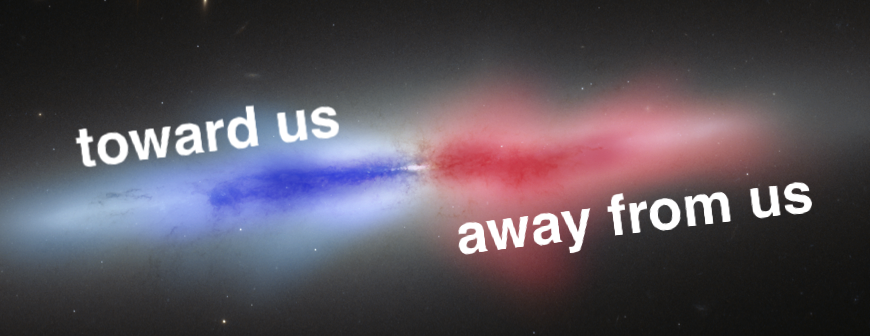
\includegraphics[width=0.6\linewidth]{pictures/toward_away.png}
\end{center}

\item Newton's law predicts orbital velocity versus distance from the
  center, assuming knowledge of the mass distribution.

(Einstein's corrections are negligible.)

\item Assume that the mass is primarily due to observed stars and gas.
\end{itemize}
\end{frame}

\begin{frame}
\frametitle{The result (same for most galaxies)}
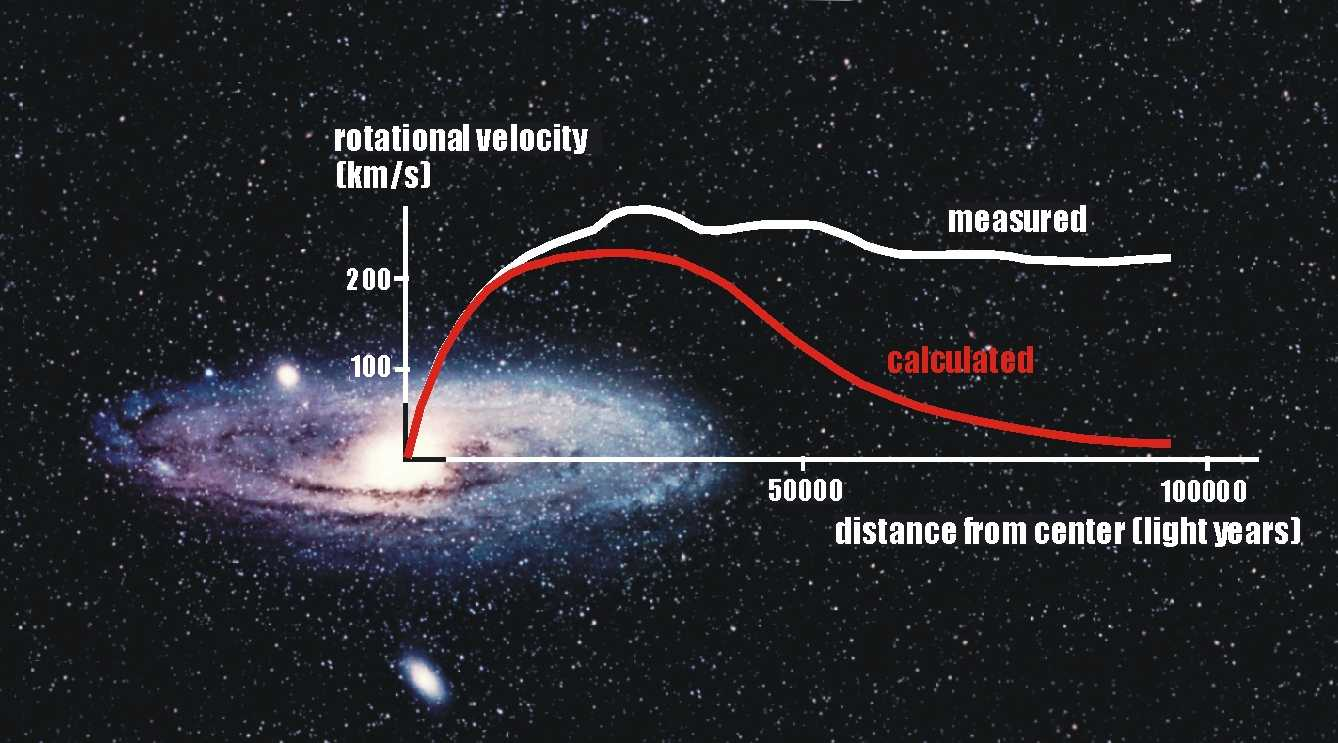
\includegraphics[width=\linewidth]{pictures/galaxy_rotation_curve.jpg}

\begin{itemize}
\item Stars are orbiting the galactic core too fast.
\item If both assumptions were valid (theory of gravity and mass
  distribution), galaxies would have spun
  apart long ago.
\end{itemize}
\end{frame}

\begin{frame}
\frametitle{What could it be?}
\begin{center}
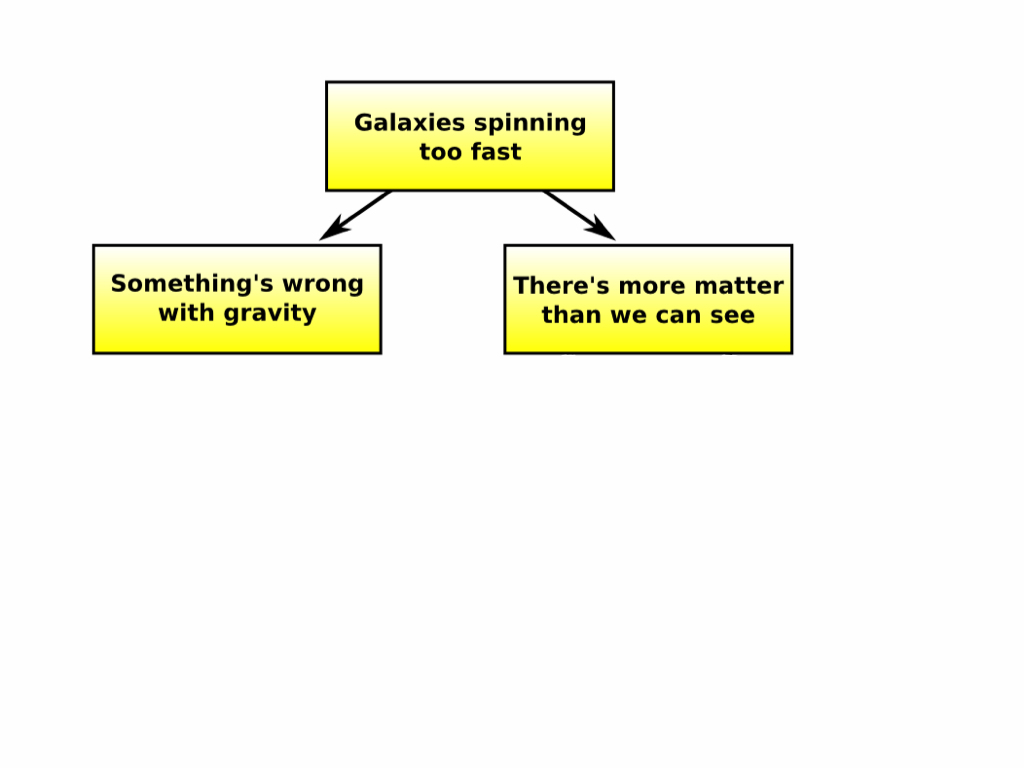
\includegraphics[width=\linewidth]{pictures/flow_chart_1.png}
\end{center}
\end{frame}

\begin{frame}
\frametitle{Modify gravity or missing matter?}

\vspace{0.2 cm}
\uncover<2>{Color: X-ray observations of hot gas (majority of normal
  matter).}

\uncover<2>{Contours: mass distribution determined from gravitational lensing.}

\begin{center}
\only<1>{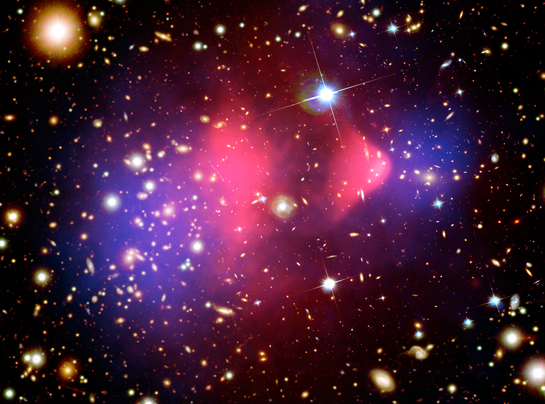
\includegraphics[width=0.85\linewidth]{pictures/bullet_cluster.jpg}}
\only<2>{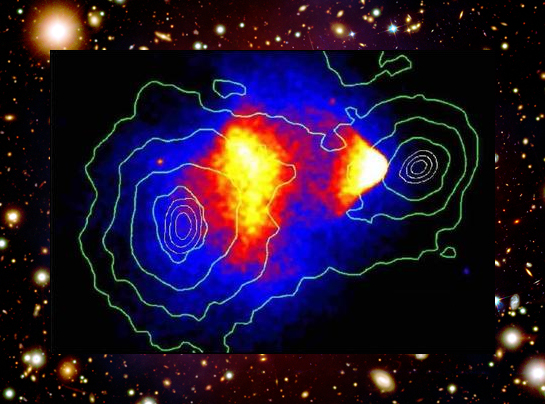
\includegraphics[width=0.85\linewidth]{pictures/bullet_cluster_overlay.jpg}}
\end{center}
\end{frame}

\begin{frame}
\frametitle{Modify gravity or missing matter?}

\begin{columns}
\column{0.75\linewidth}
\only<1>{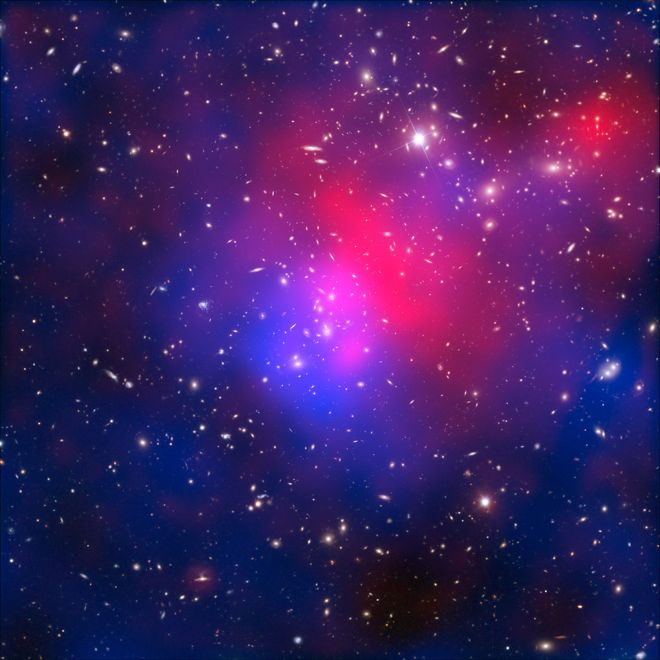
\includegraphics[width=\linewidth]{pictures/pandoras_cluster_blobs.jpg}}
\only<2>{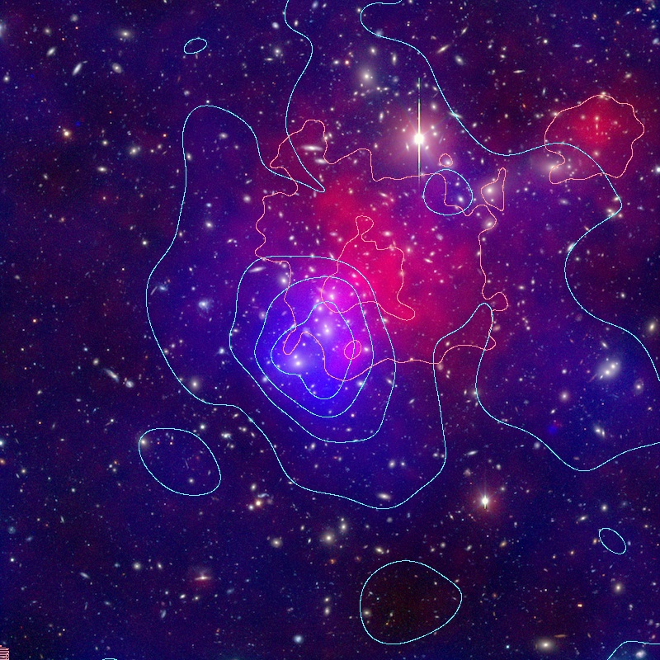
\includegraphics[width=\linewidth]{pictures/pandoras_cluster_outlines.png}}

\column{0.25\linewidth}
\uncover<2>{After colliding, most of the mass of the galaxy clusters (blue) is light
years away from the visible gas (red).}

\vspace{0.5 cm}
\uncover<2>{Strongly suggests that another {\it material} is present, not a modification
of the gas's gravitational pull.}
\end{columns}
\end{frame}

\begin{frame}
\frametitle{What could it be?}
\begin{center}
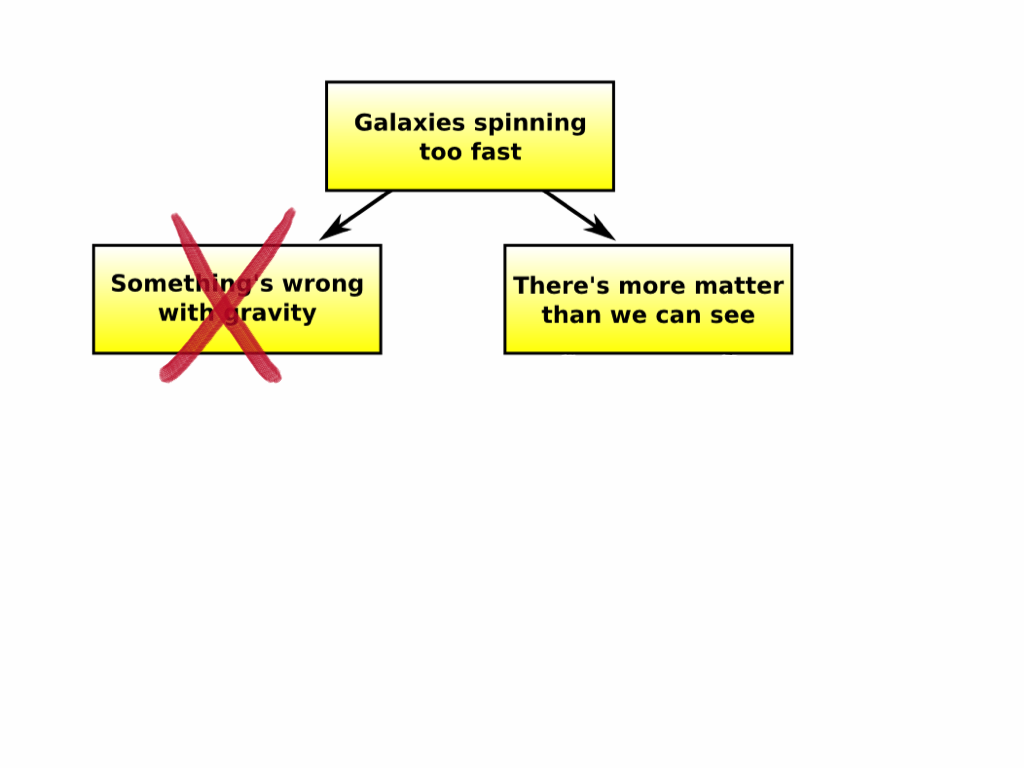
\includegraphics[width=\linewidth]{pictures/flow_chart_1_X.png}
\end{center}
\end{frame}

\begin{frame}
\frametitle{What could it be?}
\begin{center}
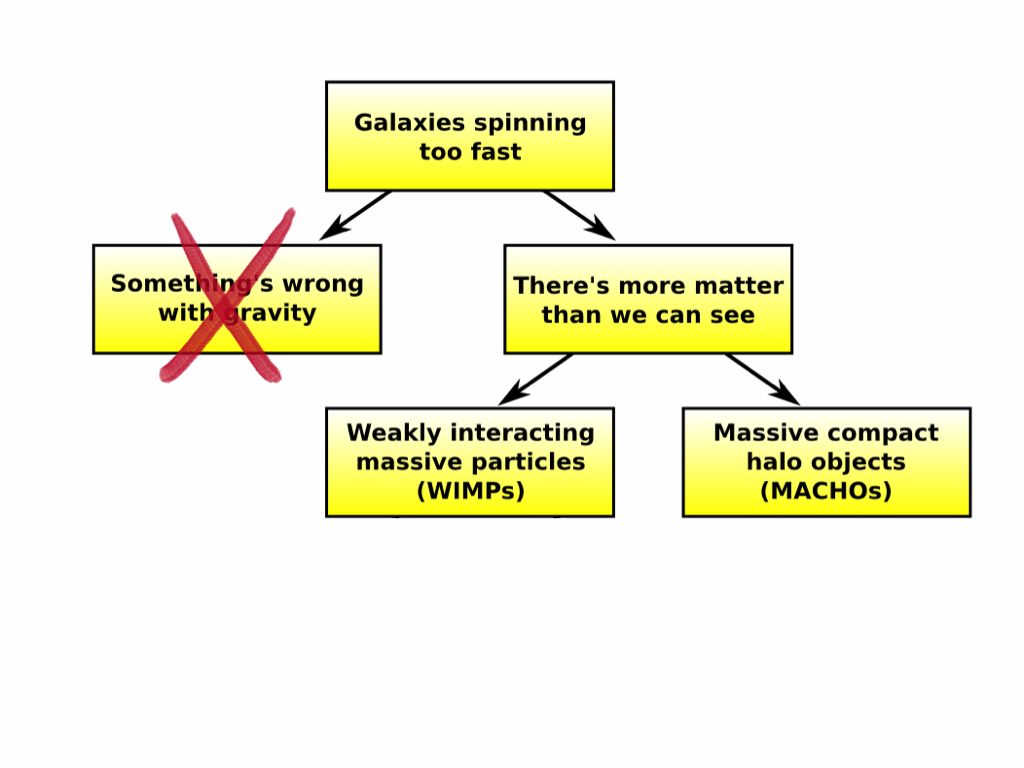
\includegraphics[width=\linewidth]{pictures/flow_chart_2.png}
\end{center}
\end{frame}

\begin{frame}
\frametitle{Massive Compact Halo Objects}
\begin{columns}
\column{0.3\linewidth}
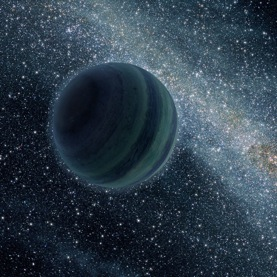
\includegraphics[width=\linewidth]{pictures/free-floating-planets-microlensing_1.jpg}
\column{0.7\linewidth}
\textcolor{darkblue}{Types of MACHOs}

\vspace{-0.2 cm}
\begin{itemize}\setlength{\itemsep}{-0.05 cm}
\item Free-floating planets and brown dwarfs
\item Old white dwarfs that have ceased glowing
\item Neutron stars
\item Black holes
\end{itemize}
\end{columns}

\vfill
\begin{columns}
\column{0.55\linewidth}
Search with microlensing: luminosity of background star briefly spikes
when a MACHO passes in front of it.

\vspace{0.25 cm}
Decades of searches, tens of microlensing events observed.

\vspace{0.25 cm}
{\it Some} of the unseen mass was due to MACHOs, but not the majority
of it.

\column{0.45\linewidth}
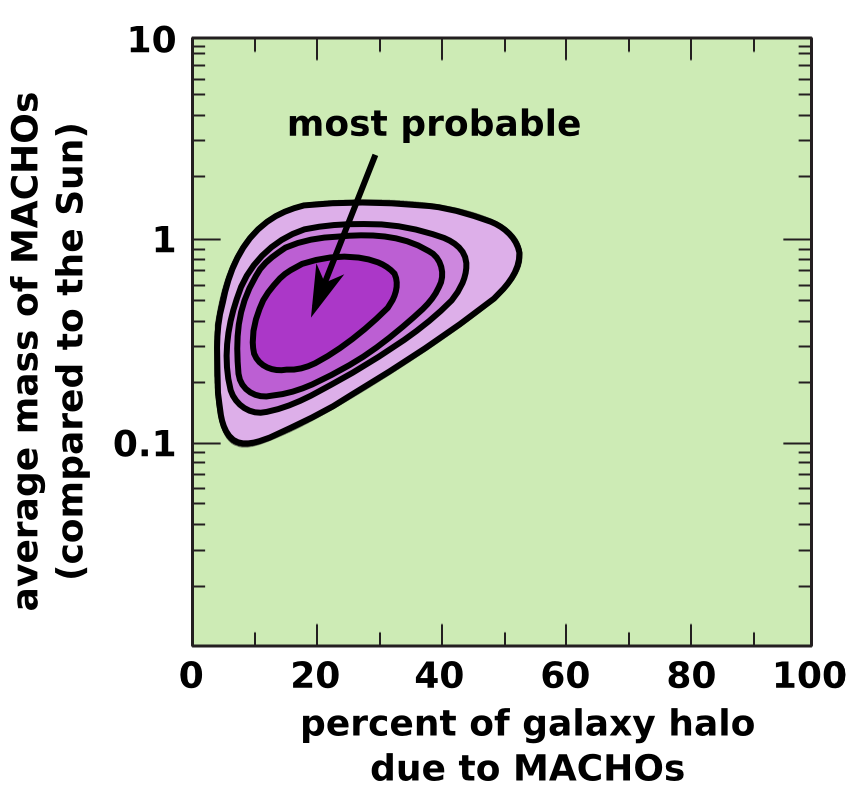
\includegraphics[width=\linewidth]{pictures/microlensing_results.png}
\end{columns}
\end{frame}

\begin{frame}
\frametitle{What could it be?}
\begin{center}
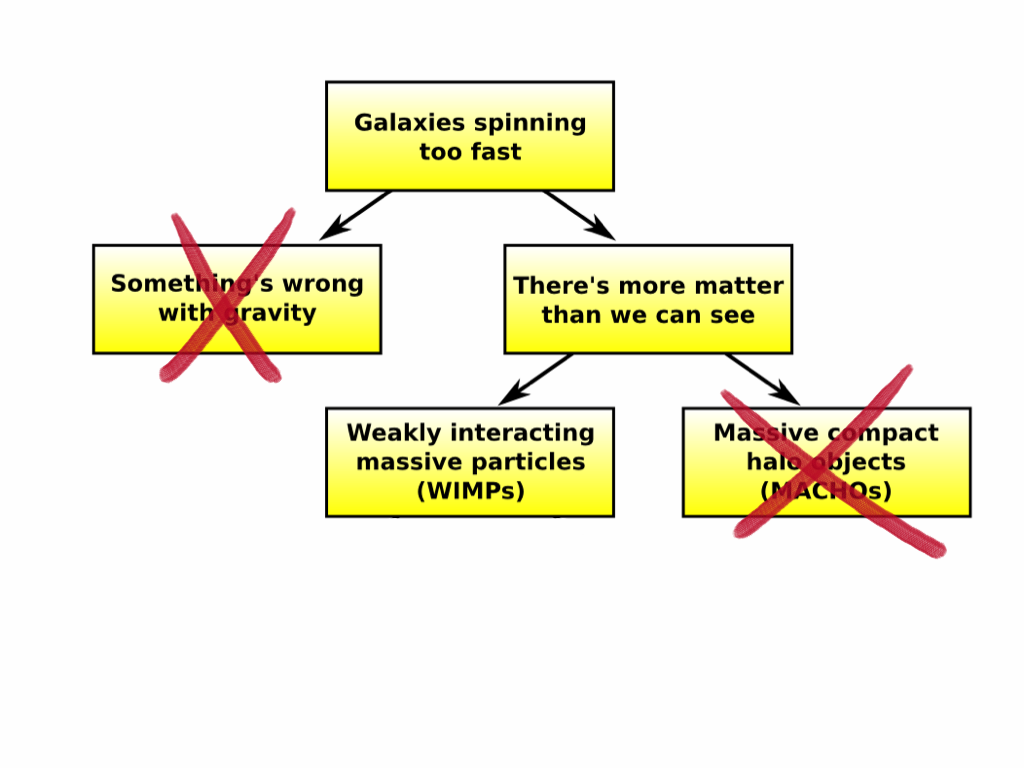
\includegraphics[width=\linewidth]{pictures/flow_chart_2_X.png}
\end{center}
\end{frame}

\begin{frame}
\frametitle{What could it be?}
\begin{center}
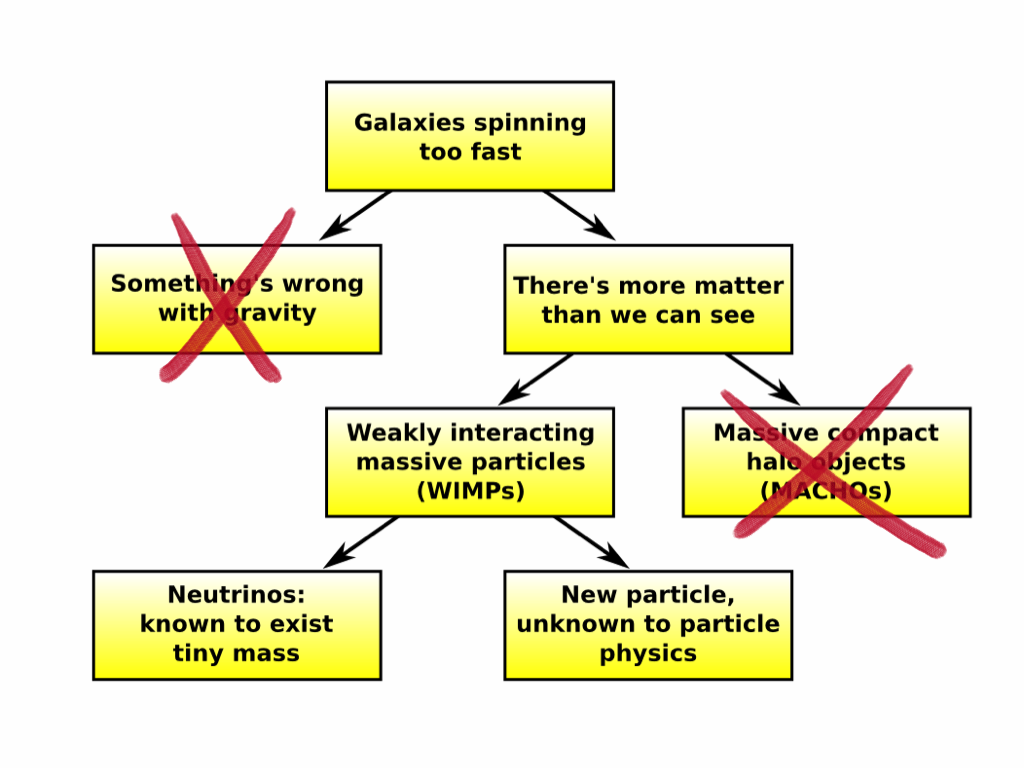
\includegraphics[width=\linewidth]{pictures/flow_chart_3.png}
\end{center}
\end{frame}

\begin{frame}
\frametitle{Neutrinos: oddballs of particle physics}

\begin{columns}
\column{0.5\linewidth}
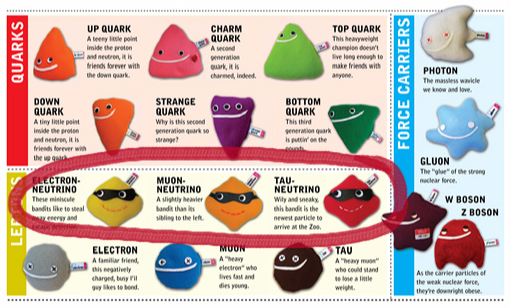
\includegraphics[width=\linewidth]{pictures/standard_model.png}
\column{0.5\linewidth}
\begin{itemize}
\item Nearly but not exactly massless, invisible, and intangible.
\item Three ``flavors,'' but spontaneously change flavor when
  travelling long distances.
\end{itemize}
\end{columns}

\vspace{0.25 cm}
\begin{itemize}
\item They probably do not travel faster than the speed of light.

  (Two errors were found in last year's apparent discovery.)

\item Hard to detect; many of their basic parameters are still unknown or not well
  known.

\item They swarm through space in vast numbers without our noticing:
  could this be the dark matter we're looking for?
\end{itemize}
\end{frame}

\begin{frame}
\frametitle{Neutrinos are too fast to be dark matter}

\begin{columns}
\column{0.35\linewidth}
Dark matter determined the development of large-scale structure
(galaxies and clusters of galaxies) in the universe.

\vspace{0.5 cm}
Neutrinos are always traveling close
to the speed of light.

\vspace{0.5 cm}
If most of the dark matter were neutrinos, they wouldn't stay put long
enough to let those structures form.

\column{0.7\linewidth}
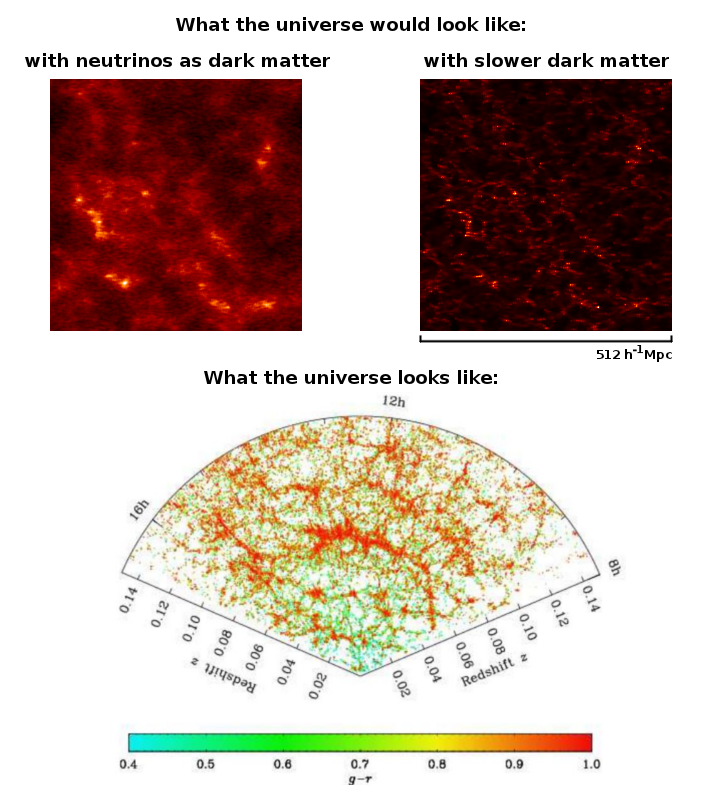
\includegraphics[width=\linewidth]{pictures/neutrinos_and_lss.png}
\end{columns}
\end{frame}

\begin{frame}
\frametitle{What could it be?}
\begin{center}
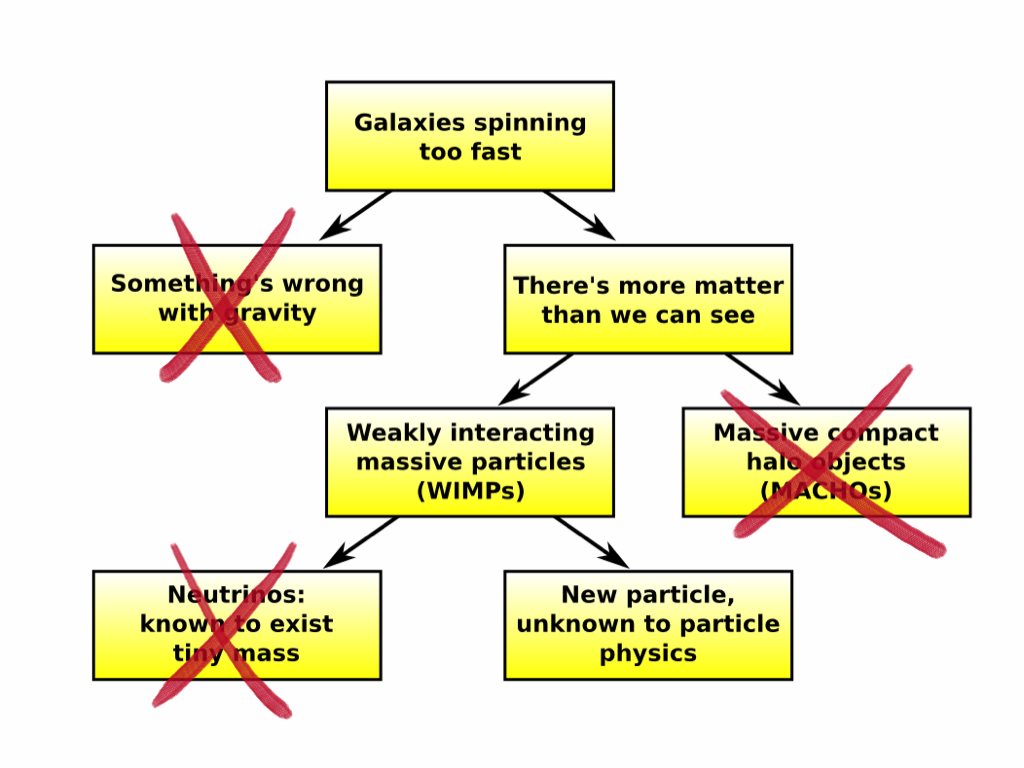
\includegraphics[width=\linewidth]{pictures/flow_chart_3_X.png}
\end{center}
\end{frame}

\begin{frame}
\frametitle{What could it be?}

\textcolor{darkblue}{The nature of dark matter is one of the foremost mysteries in physics.}

\begin{itemize}
\item Force laws obeyed:

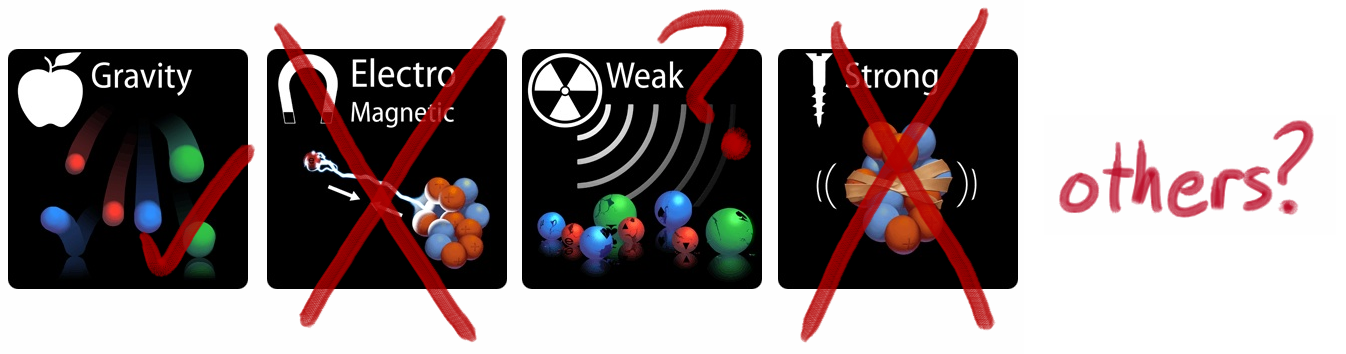
\includegraphics[width=\linewidth]{pictures/four_forces.png}

\item Speed: less than 95\% of the speed of light.

\item Mass: maybe $10^{11}$~eV (weak force scale) if thermally produced
  in the Big Bang.  Maybe as low as $10^{-5}$~eV (axion) or as high as
  $10^{19}$~eV (WIMPZILLA) if not thermally produced.

\item Connection to other mysteries of particle physics: maybe
  supersymmetry, extra dimensions, strong CP problem, inert Higgs
  doublet, sterile neutrinos, left-right symmetry\ldots
\end{itemize}
\end{frame}

\begingroup
\setbeamercolor{background canvas}{bg=black}
\begin{frame}

\mbox{\hspace{-1 cm} 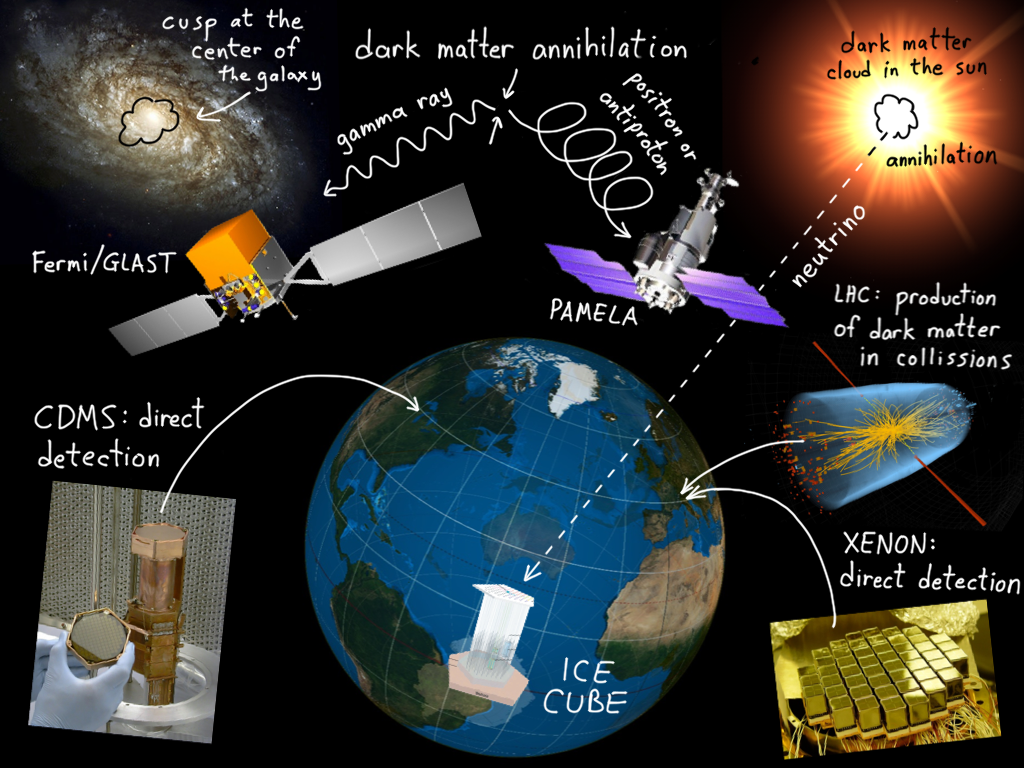
\includegraphics[width=1.17\linewidth]{pictures/experiments.png}}

\end{frame}
\endgroup

%%%%%%%%%%%%%%%%%%%%%%%%%%%%%%%%%%%%%%%%%%%%%%%%%%%%%

\section*{Dark Energy}
\begin{frame}
\begin{center}
\Huge \textcolor{blue}{Dark Energy}
\end{center}
\end{frame}

\begin{frame}
\begin{center}
\begin{minipage}{0.75\linewidth}
\vspace{0.5 cm}
Dark energy resembles dark matter in that it has ``dark'' in its name
and it's not well understood.

\vspace{0.5 cm}
\uncover<2->{This name can be applied to anything that addresses the fact that the
expansion of the universe is accelerating.}

\vspace{0.5 cm}
\uncover<3->{Universal expansion is an example of space-time
  curvature, so let's start with that.}
\end{minipage}
\end{center}
\end{frame}

\begin{frame}
\frametitle{Space-time curvature in three steps}
\framesubtitle{Step 1: Consider unusual connections between space points}

\vspace{1 cm}
\textcolor{darkblue}{\Large Normal:}

\vspace{-1.5 cm}
\begin{columns}
\column{0.5\linewidth}
\hfill 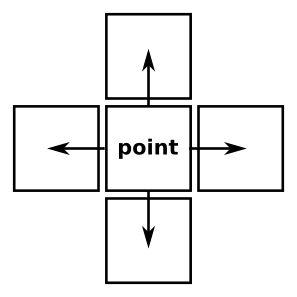
\includegraphics[width=2 cm]{pictures/normal_connections.png}

\column{0.5\linewidth}
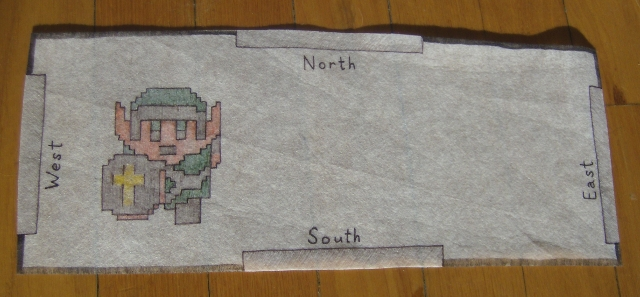
\includegraphics[width=\linewidth]{pictures/dungeon_room.jpg}
\end{columns}

\textcolor{darkblue}{\Large Unusual:}

\vspace{0.25 cm}
\begin{columns}
\column{0.5\linewidth}
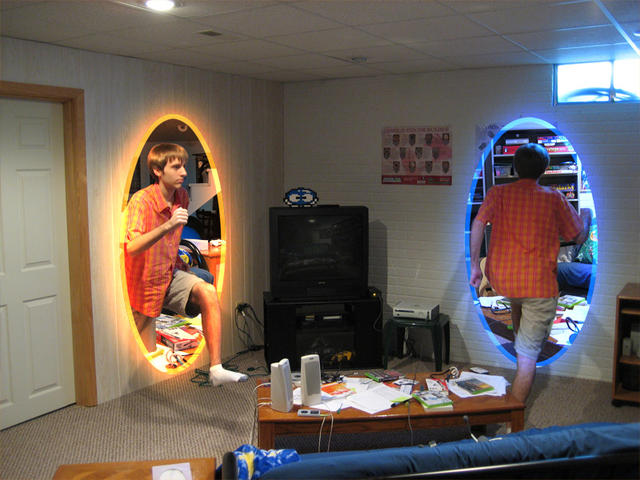
\includegraphics[width=\linewidth]{pictures/fanart_portal179.jpg}
% http://www.theverge.com/2012/2/10/2788947/Replica-portal-gun-NECA-US-release

\column{0.5\linewidth}
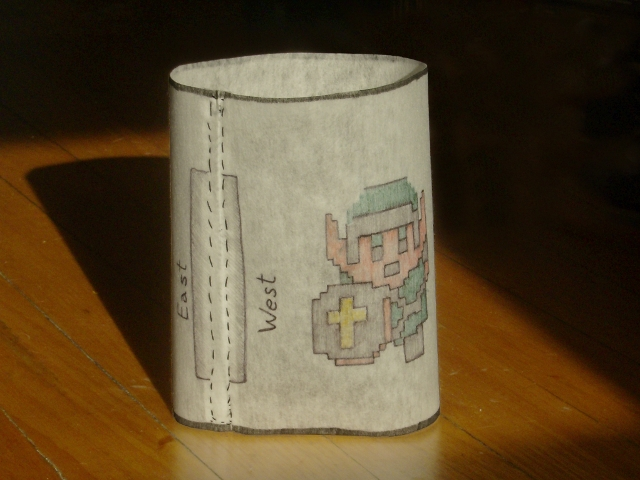
\includegraphics[width=\linewidth]{pictures/circular_dungeon.jpg}
\end{columns}
\end{frame}

\begin{frame}
\frametitle{Space-time curvature in three steps}
\framesubtitle{Step 1: Consider unusual connections between space points}

\begin{columns}
\column{0.5\linewidth}

The cloth is just a metaphor: what is important is how each point in space is connected to all of the other points in space.

\vspace{0.1 cm}
With cloth, we can sew together any stitch to any other stich.

\vspace{0.1 cm}
With space, we can only imagine it.

\vspace{0.25 cm}
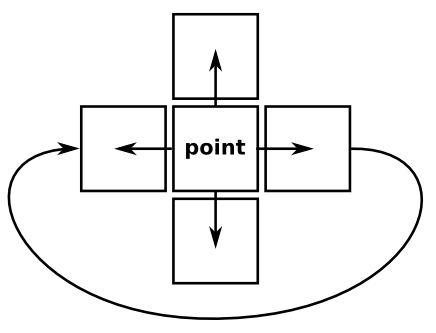
\includegraphics[width=\linewidth]{pictures/looped_connections.png}

\column{0.5\linewidth}
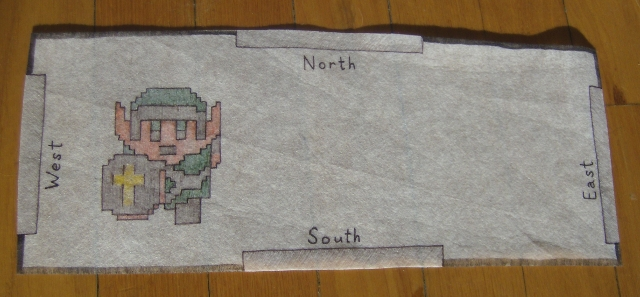
\includegraphics[width=\linewidth]{pictures/dungeon_room.jpg}

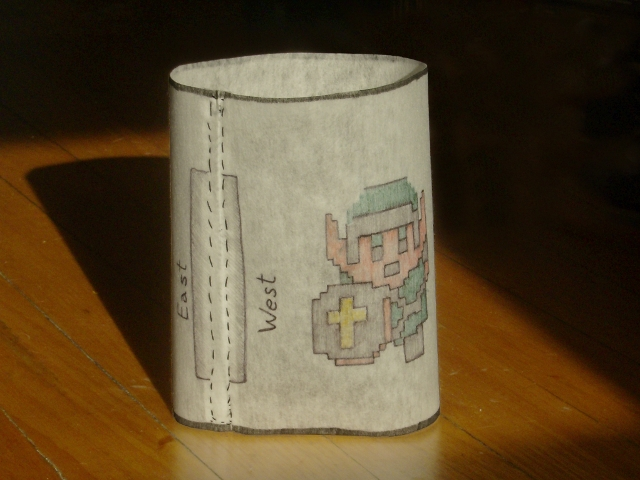
\includegraphics[width=\linewidth]{pictures/circular_dungeon.jpg}
\end{columns}
\end{frame}

\begin{frame}
\frametitle{Space-time curvature in three steps}
\framesubtitle{Step 2: Rewire nearby points with a repeating pattern}

\begin{center}
\only<1>{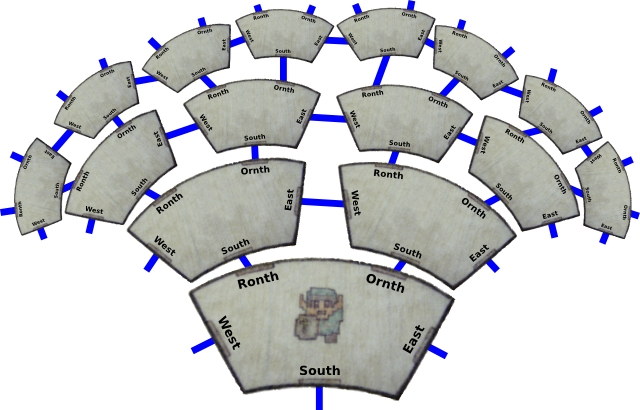
\includegraphics[width=\linewidth]{pictures/map.jpg}}
\only<2>{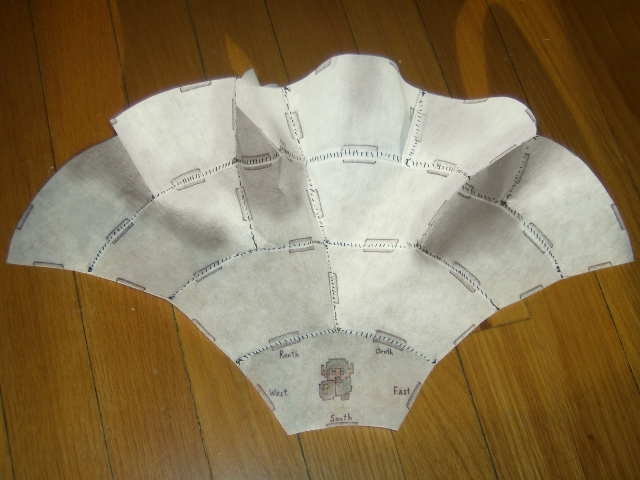
\includegraphics[width=0.95\linewidth]{pictures/curly_dungeons.jpg}}
\only<3>{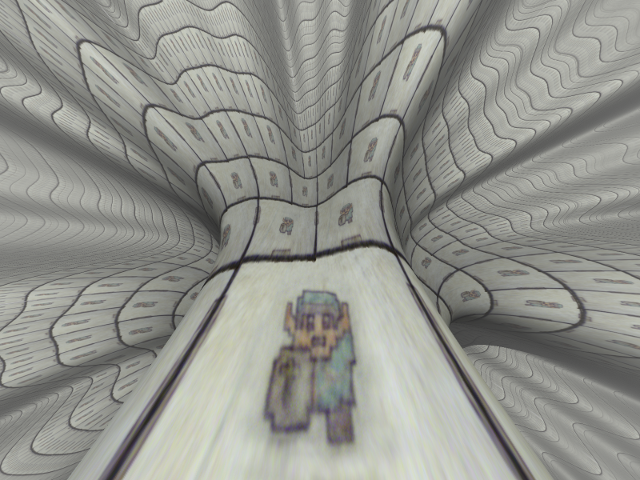
\includegraphics[width=0.95\linewidth]{pictures/linktiles.png}}
\end{center}
\end{frame}

\begin{frame}
\frametitle{Space-time curvature in three steps}
\framesubtitle{Step 3: Think of time as a dimension}

\begin{center}
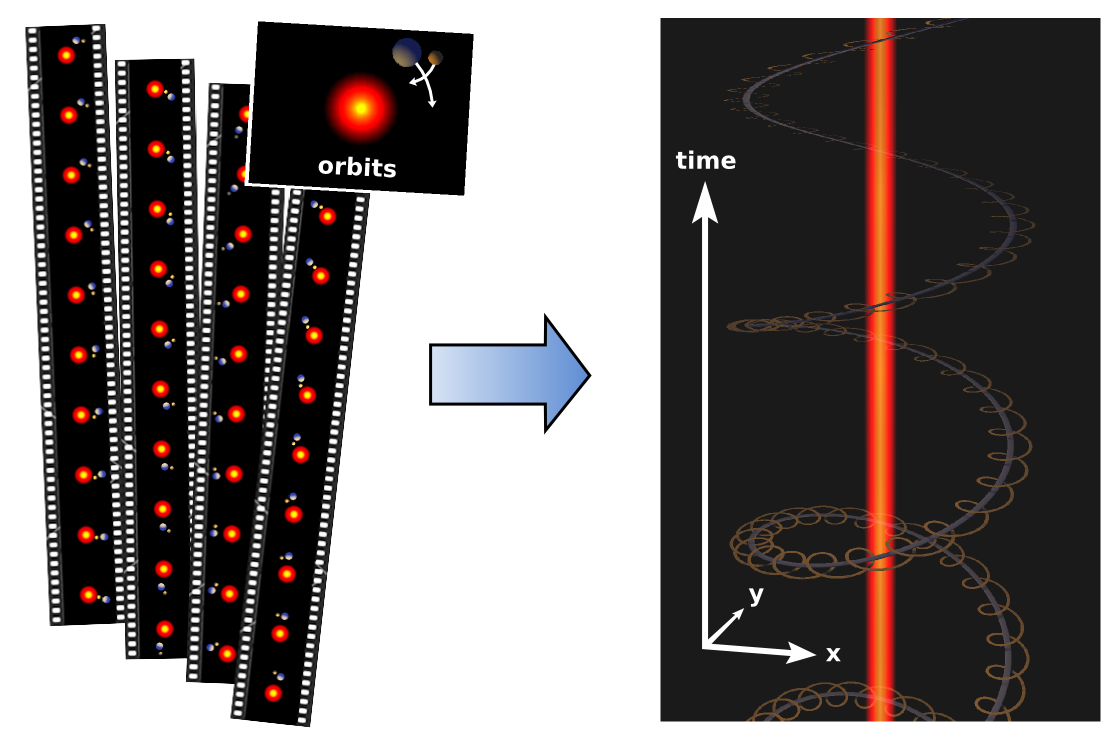
\includegraphics[width=\linewidth]{pictures/timedimension.png}
\end{center}
\end{frame}

\begin{frame}
\frametitle{Space-time curvature in three steps}
\framesubtitle{Step 3: Think of time as a dimension}

\begin{center}
\includegraphics[width=0.95\linewidth]{pictures/leap2.jpg}
\end{center}
\end{frame}

\begin{frame}
\frametitle{Space-time curvature of the early universe}

\begin{center}
\includegraphics[width=0.95\linewidth]{pictures/big_bang_manifold.png}
\end{center}
\end{frame}

\begin{frame}
\frametitle{Mapping the shape of expansion}

\begin{center}
\only<1>{\includegraphics[width=0.95\linewidth]{pictures/lightcone_diagram.png}}
\only<2>{\includegraphics[width=0.9\linewidth]{pictures/lightcone_withspeeds.png}}
\end{center}

\vspace{-0.25 cm}
\only<2>{The shape can be measured with recession speed versus distance.}
\end{frame}

\begingroup
\setbeamercolor{background canvas}{bg=black}
\begin{frame}
\begin{columns}
\column{0.4\linewidth}

\textcolor{white}{{\bf Type 1-A supernovae} are a tool for measuring distance.}

\vspace{0.1 cm}
\textcolor{white}{A white dwarf star accretes matter from its giant com- panion and explodes the moment it has acquired the critical mass.}

\vspace{0.1 cm}
\textcolor{white}{Thus, we know exactly how large and how bright it was.}

\vspace{0.5 cm}
\includegraphics[width=\linewidth]{pictures/sn1994d_circled.png}

\column{0.6\linewidth}
\centering \textcolor{white}{Artist's conception}

\vspace{0.1 cm}
\includegraphics[width=\linewidth]{pictures/type1a_supernova.jpg}
% http://www.eso.org/public/archives/images/screen/eso0731b.jpg

\vspace{0.1 cm}
\centering \textcolor{white}{Computer simulation}

\vspace{0.1 cm}
\includegraphics[width=\linewidth]{pictures/type1a_simulation.jpg}
% http://blogs.discovery.com/.a/6a00d8341bf67c53ef0162fd6caff5970d-800wi

\end{columns}
% Tycho: http://spider.seds.org/spider/Vars/sn1572.html
\end{frame}
\endgroup

\begin{frame}
\frametitle{Mapping the shape of expansion}
\includegraphics[width=\linewidth]{pictures/distance_versus_speed.png}
\end{frame}

\begin{frame}
\frametitle{Surprise: it's accelerating!}
\begin{center}
\includegraphics[width=0.95\linewidth]{pictures/newinflation.png}
\end{center}
\end{frame}

\begin{frame}
\frametitle{Surprise: it's accelerating!}
\begin{center}
\includegraphics[width=\linewidth]{pictures/physicstoday_expansion.jpg}
\end{center}
\end{frame}

\begin{frame}
\vspace{0.5 cm}
\begin{columns}
\column{0.3\linewidth}
\includegraphics[width=\linewidth]{pictures/newinflation.png}
\column{0.7\linewidth}
\textcolor{darkblue}{\Large Accelerating expansion: what could it mean?}
\end{columns}

\vspace{0.25 cm}
\begin{itemize}\setlength{\itemsep}{0.25 cm}
\item Matter curves space-time in such a way that massive objects move toward each other (gravity).

\item From all the matter in the universe, including dark matter, we would expect the universe to curve inward: {\it decelerating} expansion.
\end{itemize}

\begin{center}
\includegraphics[width=\linewidth]{pictures/darkenergy_flow_chart.png}
\end{center}
\end{frame}

\section*{Shameless plugs}

\begin{frame}
\frametitle{Dark Energy Survey, built at Fermilab}

\vspace{-0.25 cm}
\begin{itemize}
\item Survey telescope to study dark matter and dark energy:
\begin{itemize}
\item count galaxy clusters and use gravitational lensing to map the
  mass/dark matter distribution,
\item collect thousands of supernovae to map expansion history.
\end{itemize}

\item Extremely wide field of view: 2.2 degrees, extremely deep: 570
  megapixel camera, extremely fast: 17 seconds per image.

\item Camera is being installed in Chile {\it right now.}
\end{itemize}

\begin{columns}
\column{0.5\linewidth}
\centering \scriptsize building the camera at Fermilab

\includegraphics[width=0.9\linewidth]{pictures/deccam.jpg}

\column{0.5\linewidth}
\centering \scriptsize Blanco observatory in Chile

\includegraphics[width=0.9\linewidth]{pictures/blanco.jpg}
\end{columns}
\end{frame}

\begin{frame}
\frametitle{http://www.coffeeshopphysics.com}

\vspace{0.25 cm}
\includegraphics[width=\linewidth]{pictures/coffeeshopphysics.png}
\label{numpages}
\end{frame}

\end{document}
